\documentclass[a4paper]{article}

\usepackage[utf8]{inputenc}
\usepackage[portuges]{babel}
\usepackage{fullpage} % Package to use full page
\usepackage{parskip} % Package to tweak paragraph skipping
\usepackage{tikz} % Package for drawing
\usepackage{amsmath}
\usepackage{hyperref}
\usepackage{bm}
\usepackage{graphicx}
%\graphicspath{ {./images/} }

\newcommand{\sample}[2]{
    \begin{center}
        \begin{tabular}{ | c | c | }
            \hline
            Entrada & Saída \\ \hline
            \begin{minipage}{0.4\textwidth}#1\end{minipage} & \begin{minipage}{0.4\textwidth}#2\end{minipage} \\ \hline
        \end{tabular}
    \end{center}
}

\title{Maximização de Lucro em Radares por Máquina de Turing}
\author{
  Bernardo Flores Salmeron\\
  \and
  Denilson das Mercês Amorim\\
  \and
  Lucas Natanael Brito Prates\\
  \and
  Thalles Yan Santos Medrado
}
\date{26/11/2018}

\begin{document}

\maketitle

%Aqui vamos enunciar o problema
\section{Introdução}

Máquina de Turing é um modelo matemático de computação definindo uma máquina abstrata operando em símbolos de uma fita de acordo com uma tabela de regras. Introduzido em 1936 por Alan Turing, o modelo é capaz de expressar qualquer algoritmo de computador.

Neste trabalho é apresentado uma máquina de Turing capaz de resolver o problema da maximização de lucro em radares. O problema foi adaptado do URI Online Judge\cite{uriproblem}.

\section{Problema}

%O problema consiste em encontrar a melhor distribuição de radares em uma rodovia de forma que a arrecadação seja maximizada. Porém esse arranjamento deve respeitar a seguinte regra: A distância entre quaisquer dois radares deve ser de no mínimo $K$ posições.

Dado o lucro obtido ao se instalar um radar em cada ponto de uma rodovia, qual lucro máximo pode-se obter dado que quaisquer dois radares devem estar separados por no mínimo $K$ posições?


    \subsection{Entrada}
       A entrada contém dois números $N$ e $K$ $(1 \leq K \leq N)$ — o tamanho da rodovia e a distância mínima entre dois radares, respectivamente. Em seguida, a entrada contem $N$ números $lucro_{1}, lucro_{2}, \dots, lucro_{N}$ $(lucro_{i} \geq 1)$ correspondentes ao lucro de instalação de um radar na i-ésima posição.
       
       Os números da entrada são representados no sistema unário e são separados por um espaço em branco.

    \subsection{Saída} 
        A saída deve ser a arrecadação máxima correspondente a melhor distribuição de radares.
    
    \subsection{Exemplo}
    \sample{11111\_11\_111\_11\_11111\_111\_111}{11111111111}

\section{Algoritmo}

O problema apresenta subestrutura ótima e, portanto, pode ser resolvido por programação dinâmica. O subproblema ótimo usando na resolução de problemas maiores é: Qual melhor lucro pode-se obter (dada a restrição) até uma certa posição $i$ $(0 \leq i \leq N)$ da rodovia?

A seguinte recorrência é capaz de solucionar o problema:

$\qquad\operatorname{rad}_k(i) = \begin{cases}
  0 & \text{ se } i=0, \\
  \max \begin{cases}
          \operatorname{rad}_k(i-1) \\
          \operatorname{rad}_k(\max(0, i-k)) + lucro_i
       \end{cases} & \text{ caso contrário.}
\end{cases}$

\bigskip
Em palavras simples:
\begin{itemize}
\item Na posição zero (i.e. não existe rodovia), não é possível obter lucro.
\item Nas demais posições, maximiza-se a escolher entre não inserir o radar $i$ e manter o lucro até o momento, ou inserir o radar $i$ e acumular o $lucro_i$ ao melhor lucro até a $k$-ésima posição anterior.
\end{itemize}

Essa recorrência pode ser convertida em um algoritmo iterativo com o auxílio de uma tabela de recorrência $dp[0...N]$.

\begin{enumerate}
\item Inicialize $dp[0]$ com $0$.
\item Para cada $i$ entre $1$ e $N$ (inclusivo), inicialize $dp[i]$ com o máximo entre $dp[i-1]$ e $dp[\max(0, i-k)] + lucro_i$.
\item Feito isso, a solução para o problema encontra-se em $dp[N]$.
\end{enumerate}

\section{Implementação}

A implementação da máquina final foi dividida pela equipe em três etapas.

\subsection{Abstração}

Nesta etapa a equipe abstraiu a máquina final como um conjunto de Máquinas de Turing. Para isso, a implementação da máquina foi dividida em subproblemas de modo a simplificar a ideia e cada tarefa foi implementada individualmente em diferentes estados. Para esse problema, foi utilizada uma máquina de sete fitas e $35$ estados. As fitas foram distribuídas da seguinte maneira: 

\begin{enumerate}
\item Fita I/O: Recebe o valor de entrada e imprime o valor de saída
\item Fita N: Contém o tamanho da rodovia
\item Fita K: Contém a distância máxima permitida entre rodovias
\item Fita I: Controla o iterador I do laço utilizado na solução
\item Fita DP: Contém o vetor DP e seus respectivos valores em ordem crescente de índice
\item Fita X1: Fita auxiliar para realizar operações
\item Fita X2: Fita auxiliar para realizar operações
\end{enumerate}

\medskip
Um diagrama da maquina pode ser encontrado na Figura~\ref{fig:image}.

%\begin{figure}
%    \centering
%    \def\svgwidth{\columnwidth}
%    \input{image.pdf_tex}
%\end{figure}

\pagebreak
\begin{figure}[h]
\centering
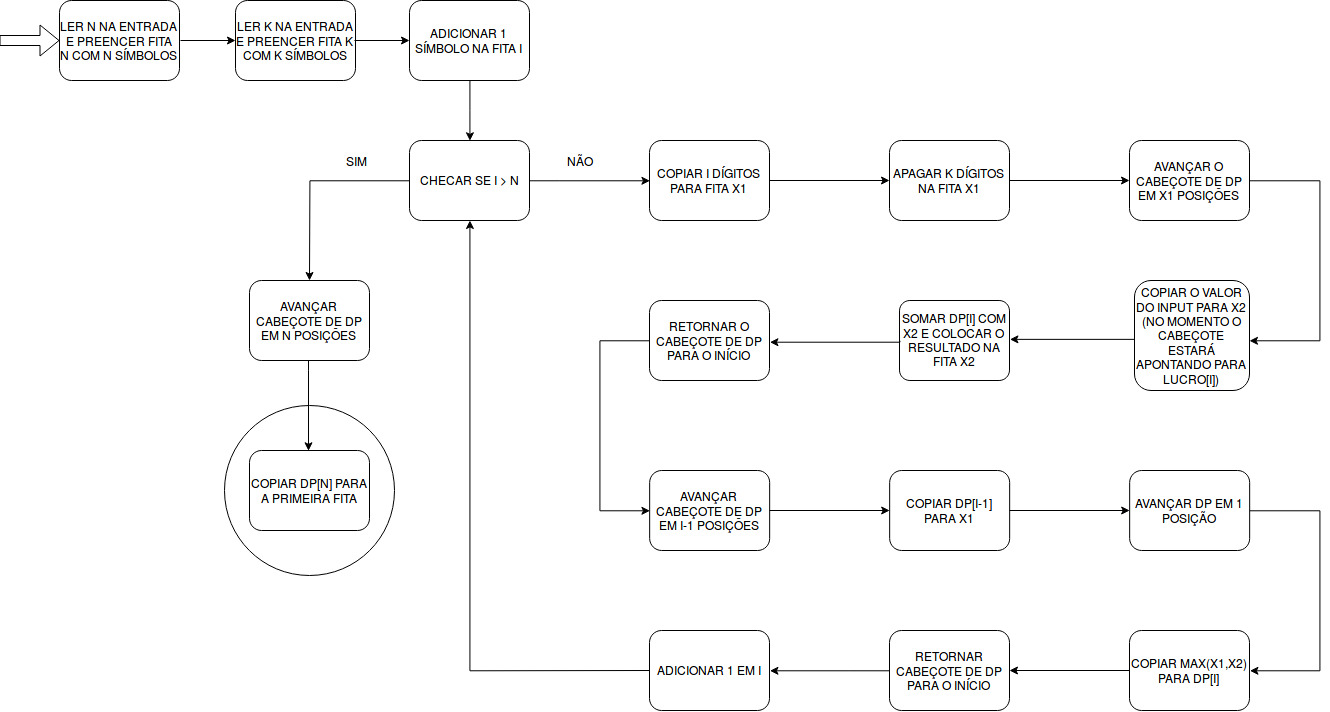
\includegraphics[scale=0.30]{turing.jpg}
\caption{Diagrama da Máquina de Turing}
\label{fig:image}
\end{figure}

\subsection{Linguagem Simples}

Como a máquina final tem sete fitas, notou-se que seria uma atividade complexa e exaustiva criar todas as permutações de transições requeridas pelo simulador de Máquinas de Turing quando a maioria das transições realizavam operações simples sobre no máximo três fitas.

Visando diminuir o trabalho manual desnecessário, a equipe optou por criar e utilizar uma linguagem mais simples baseada na linguagem do simulador, que é posteriormente convertida na linguagem base.

Nessa linguagem:
\begin{itemize}
    \item As palavras chaves padrões do simulador (\textit{name}, \textit{init}, \textit{accept}), bem como suas funções, foram mantidas.
    \item Uma palavras chaves \textit{fitas} foi adicionada e sua função é definir a quantidade, os $id$s e a ordem das fitas. Isso significa que essa palavra chave deve ser seguida por $N$ $id$s (representando $N$ fitas) separados por vírgula, onde o $i$-ésimo $id$ representa a $i$-ésima fita da máquina final.
    \item Houve uma leve, mas importante, modificação na definição de transições que agora seguem o seguinte padrão:

    $//[current\_tape]^M$

    $[current\_state],[read\_symbol]^M$

    $[new\_state],[write\_symbol]^M,[>|<|-]^M$
    
    Nessa nova definição, $M$ é a quantidade de fitas nas quais se deseja realizar uma operação. $[current\_tape]^M$ define a ordem de leitura e escrita das fitas que são modificadas nessa transição, i.e. $[read\_symbol]^M$[$i$] representa o símbolo que deve ser lido na fita de $id$ $[current\_tape]^M$[$i$] para $0 < i < M$ (o mesmo vale para os símbolos a serem escritos e as operações a serem realizadas). As demais $N-M$ fitas não serão modificadas, i.e. são geradas todas as permutações dessa transição adicionando as outras fitas sem modifica-las (lendo 1, escrevendo 1 e ficando ou lendo 0, escrevendo 0 e ficando).
    \item \textit{?} foi definido como símbolo especial de leitura e escrita.
    
    Numa transição, caso uma fita tenha como $[read\_symbol]$ e $[write\_symbol]$ \textit{?}, serão adicionadas permutações dessa transição (lendo 1 e escrevendo 1 ou lendo 0 e escrevendo 0) realizando a operação definida na transição para a respectiva fita.
    \item Adotou-se $//--$ como símbolo que inicia uma linha de comentário (ignorada).
\end{itemize}

\subsection{Parser}

Nesta última etapa foi realizada a implementação da máquina na linguagem simples que foi posteriormente convertida na linguagem do simulador (através de um parser simples e objetivo escrito em Python 3 e baseado em expressões regulares).

\section{Conclusão}

Nesse trabalho avaliamos o poder computacional do modelo de Máquinas de Turing através da implementação de um algoritmo de programação dinâmica.

O modelo mostrou-se poderoso, porém complicado, produzindo maquinas com milhares de transições, necessitando de um passo intermediário na sua construção.


\medskip
\begin{thebibliography}{9}
\bibitem{uriproblem} 
Radares - URI Online Judge,
\\\texttt{https://www.urionlinejudge.com.br/judge/pt/problems/view/1689}
\end{thebibliography}
\end{document}